\documentclass[tikz,border=8pt]{standalone}
% Shared look for every TikZ diagram. Load with \input{../../tools/tikz-style.tex}
\usepackage[T1]{fontenc}
\usepackage{lmodern}
\renewcommand{\sfdefault}{lmr}  % diagrams use the same serif as the text
\usetikzlibrary{arrows.meta, positioning, shapes.geometric, calc, fit, backgrounds}
\definecolor{cblue}{HTML}{4C78A8}
\definecolor{corange}{HTML}{F58518}
\definecolor{cgreen}{HTML}{54A24B}
\definecolor{cred}{HTML}{E45756}
\definecolor{cpurple}{HTML}{B279A2}
\definecolor{cgrey}{HTML}{6B6B6B}
\tikzset{
  every picture/.style={font=\sffamily, line width=1.2pt},
  box/.style={draw=#1, fill=#1!12, rounded corners=4pt, align=center, inner sep=7pt, minimum height=1.1cm},
  box/.default=cgrey,
  arrow/.style={-{Stealth[length=3mm]}, draw=cgrey, line width=1.4pt},
  title/.style={font=\sffamily\bfseries\Large},
  note/.style={font=\sffamily\small, text=cgrey, align=center},
}
\AtBeginDocument{\hyphenpenalty=10000 \exhyphenpenalty=10000}

% Two robots at (2, 1) drive forward at 0.5 m/s for 1 s: facing along x it ends at (2.5, 1), facing along y at (2, 1.5).
\begin{document}
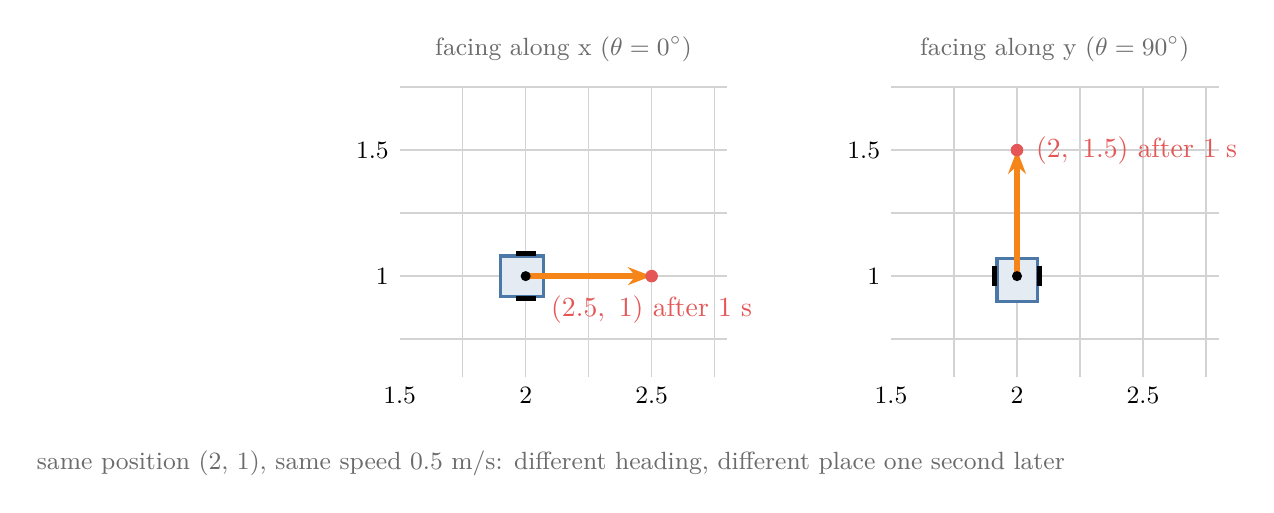
\begin{tikzpicture}[scale=3.2, every node/.append style={font=\large}]
  \foreach \panel/\ang/\ex/\ey/\lab/\pos in {0/0/2.5/1/{facing along x ($\theta = 0^\circ$)}/below, 1/90/2/1.5/{facing along y ($\theta = 90^\circ$)}/right} {
    \begin{scope}[xshift=\panel*1.95cm]
      \begin{scope}[shift={(-1.5,-0.6)}]
        \draw[cgrey!30, line width=0.5pt] (1.5,0.6) grid[step=0.25] (2.8,1.75);
        \node[note] at (2.15,1.9) {\lab};
        \foreach \t in {1.5,2,2.5} \node[below, font=\small] at (\t,0.6) {\t};
        \foreach \t in {1,1.5} \node[left, font=\small] at (1.5,\t) {\t};
        \begin{scope}[shift={(2,1)}, rotate=\ang]
          \draw[cblue, fill=cblue!15] (-0.1,-0.08) rectangle (0.07,0.08);
          \fill[black] (-0.04,0.08) rectangle (0.04,0.1); \fill[black] (-0.04,-0.1) rectangle (0.04,-0.08);
        \end{scope}
        \draw[-{Stealth[length=3mm]}, corange, line width=2pt] (2,1) -- (\ex,\ey);
        \fill[cred] (\ex,\ey) circle (0.025);
        \node[cred, \pos=3pt, font=\normalsize] at (\ex,\ey) {$(\ex,\ \ey)$ after 1 s};
        \fill[black] (2,1) circle (0.02);
      \end{scope}
    \end{scope}
  }
  \node[note, anchor=north] at (0.6,-0.25) {same position (2, 1), same speed 0.5 m/s: different heading, different place one second later};
\end{tikzpicture}
\end{document}
